\documentclass[conference]{IEEEtran}

\usepackage[utf8]{inputenc}
\usepackage[T1]{fontenc}
\usepackage{silence}\WarningsOff[latexfont]

\usepackage{amsmath}

\RequirePackage{tikz}[2010/10/13]
\usetikzlibrary{arrows,automata,calc,intersections,patterns,decorations.pathmorphing,decorations.pathreplacing}

\usepackage{graphicx}
\usepackage{cite}
\usepackage{url}
\usepackage[caption=false,font=footnotesize]{subfig}
\usepackage[binary-units,per-mode=symbol]{siunitx}
\sisetup{list-final-separator = {, and }}
\usepackage{booktabs}
\usepackage{pifont}
\usepackage{microtype}
\usepackage{textcomp}
\usepackage[american]{babel}
\usepackage[noabbrev,capitalise]{cleveref}
\usepackage{xspace}
\usepackage{hyphenat}
\usepackage[draft,inline,nomargin,index]{fixme}
\fxsetup{theme=color}
\usepackage{grffile}
\usepackage{xfrac}
\usepackage{multirow}
\RequirePackage{xstring}
\RequirePackage{xparse}
\RequirePackage[index=true]{acro}
\NewDocumentCommand\acrodef{mO{#1}mG{}}{\DeclareAcronym{#1}{short={#2}, long={#3}, #4}}
\NewDocumentCommand\acused{m}{\acuse{#1}}
\usepackage{upquote}
\usepackage{comment}

\acrodef{WSN}{Wireless Sensor Network}
\acrodef{MANET}{Mobile Ad Hoc Network}
\acrodef{ROI}{Region of Interest}{short-indefinite={an}, long-plural-form={Regions of Interest}}

\begin{document}

\title{Implementing Virtual Synchrony in a P2P group communication}

\author{
	\IEEEauthorblockN{Piermaria Arvani, S198465, \texttt{piermaria.arvani@studenti.unitn.it}}
	\IEEEauthorblockN{Lorenzo Brugnera, S197054, \texttt{lorenzo.brugnera@studenti.unitn.it}}
}

\maketitle

\begin{abstract}
The project consists of developing a system using Akka. The actors
taking part in the system are called Akka actors and they are able
to exchange of messages between each other under some conditions.
Each peer is both able to send and deliver multicast messages and 
the overall system is fault tolerant in case of silent crash from
a group member.   

\begin{comment}
	Quickly describe what your work is about, what you have been doing, what are the main conclusions.
The abstract is normally present in long reports, if your report is 1--3 pages you can avoid it as reading the entire document is not a major effort. 
\end{comment}
\end{abstract}

\section{Introduction}
\label{sec:introduction}
The project aims at showing a simple message exchange mechanism between
peers belonging to the same group. The actors taking part in the group
can be of two types:
\begin{itemize}
	\item \textbf{Manager}
	\item \textbf{Partecipant}
\end{itemize} 
The group manager is reliable, responsible for serializing group view
changes and sending view updates to all the participants. 
Furthermore, it is also able to detect silent crashes and initiate view
changes to notify the other members that the group has changed.\\
The exchange of messages is governed by the \texttt{Virtual Synchrony}
protocol, which ensures first that the communication between actors is
consistent and secondly that the system is fault tolerant in case of
silent crash of one or more actors taking part in the message exchange.


\begin{comment}
\begin{itemize}
\item general motivation for your work, context and goals.
\item problem: what is the problem you are trying to address, solve, or reason on?
\item strategy: the way you will address the problem
\end{itemize}	
The introduction or first section can also have a different title if you think another one represents better the content. 

Don't write obvious/silly things like ``This is the report of Assignment No.\ 1,'' or cut \& paste here parts of the assignment. 

\end{comment}


\begin{comment}
\section{Fundamentals / Theory / Basic Information / \ldots}
\label{sec:fundamentals}

\begin{itemize}
\item describe methods and techniques that build the basis of your work
\item include what's needed to understand your work (e.g., techniques, protocols, models, hardware, software, ...)
\item exclude what's not (e.g., anything you yourself did, anything your reader can be expected to know, ...)
\end{itemize}	
\end{comment}

\section{Implementation}
The overall system has been developed in Akka. Akka provides a higher
level of abstraction for writing concurrent and distributed systems. \\
The code is structured in two java classes:
\begin{itemize}
	\item \textbf{CausalMulticast.java}, which represents the main 
	\item \textbf{Chatter.java}, which represents all the logic behind
	the system
\end{itemize}
Every message being exchanged in the communication has a specific
structure according to the needed information to spread around. 
All the message types are implemented by \texttt{public static classes}
implementing the \texttt{Serializable} interface.\\
To maintain information about the view and all the actors taking part
in that specific view, we defined a data structure called \texttt{Groups}.
Every Groups instance is composed by the view, IDs and the list of the
actors partecipating to that view. \\
In order to better understand the functioning of the system, the 
following flow graphs give the main idea. \\
\begin{figure}[ht]%
	\centering
	\subfloat{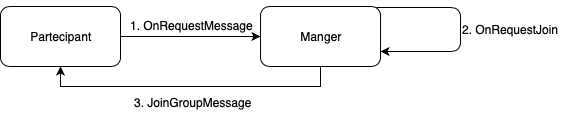
\includegraphics[width=\columnwidth]{figures/joinRequest.png}}\\%
	\caption{The graps shows the flow of execution when a participant
	wants to join an existing group}%
	\label{fig:join}%
\end{figure}
Figure \ref{fig:join} shows whenever a partecipant wants to join a 
group. First, it contacts the manager. The latter elaborates the
request and, eventually, it adds the new peer to the group by sending
him a new JoinGroupMsg containing the unique ID of the new member. \\
The Figure \ref{fig:NewView} shows the flow of execution to instantiate a new view.
Whenever a new join request or a silent crash occurs, the manager
receives respectively either a RequestJoinMsg or a TimeoutMsg.
Afterwords, it instantiates the view change process and,
eventually, all the peers receives the message and execute the flush
protocol. This protocol is needed to make all the participants aware
that they have received all unstable messages from all the members
in the group.
Only after having received the flush message from all the peers, the 
group members are allowed to install the new view. \\
\begin{figure}[ht]%
	\centering
	\subfloat{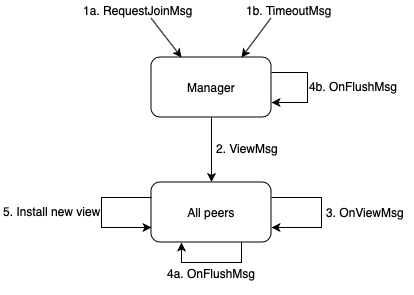
\includegraphics[width=\columnwidth]{figures/NewView.png}}\\%
	\caption{The graph shows the flow of execution when a new view has
	to be instantiated}%
	\label{fig:NewView}%
\end{figure}
In order to exchange messages, a peer has to have installed the most 
recent view. Simply, in the code this is shown by the
\texttt{inhibit\_sends} field, which has to be zero in order to allow 
the exchange of messages. \\
Another important scenario to be described is the silent crash detection
mechanics. The implementation takes place through a simple beacon mechanism:
every five seconds each peer has to send a beacon to the manager, 
indicating that specific peer is still alive. Since the channel 
is reliable, as soon as the manager does not receive even a single beacon from 
a participant, the group manager receives a \texttt{TimeoutMsg}
indicating that a silent crash occured. In particular, he is able to understand
which peer crashed, thanks to a dedicated data HashMap where the pair key-value
is represented by the peer and a \texttt{Cancellable} object. The latter object 
is used to update the time in which the that specific peer sent the beacon.
Afterwords, the manager instantiates a new view without the crashed node.\\
Moreover, there are some supporting functions used to simplify the overall
application. 



\begin{comment}
\begin{itemize}
\item describe everything you yourself did (as opposed to the fundamentals section, which explains what you built on)
\item explain the mathematical framework (if any)
\item explain your model
\item describe the developed system/algorithm/method
\end{itemize}
\end{comment}

\section{Conclusion}
This project suggests a simple implementation of a distributed application
according to the protocol. Everything works properly ad the overall system
is very easily tesatble. 

\begin{comment}
	\begin{itemize}
\item summarize again what your work did, but now emphasize more the results
\item write conclusions that can be drawn from the results found and the discussion presented in the work
\end{itemize}
Again for very short documents the conclusions can be embedded with the last section, but this depends on the structure you give to your document. 

\end{comment}


\bibliographystyle{IEEEtran}
\bibliography{references}

\section{Appendix: \LaTeX\xspace Tips}

\subsection{Cross References}
\label{sec:cross-ref}

\begin{comment}
	Cross references are an easy way to point a reader to certain parts of the text.
For figures, tables, and equations, they are a must.
Use the \verb|\cref| command to make references to a label.
For example, if you use \verb|\label{eq:newton-second}| to label the following formula
\begin{equation}
	\vec{F} = m\vec{a}\label{eq:newton-second}
\end{equation}
you can than refer to that in the text using \verb|\cref{eq:newton-second}|.
Example: The formula in \cref{eq:newton-second} is known as Newton's second law of motion.

\end{comment}


%\section{Algorithms}
%
%Use algorithms to explain what would be too hard to express in the text body of your thesis.
%
%For example: Based on the periodically transmitted \texttt{hello} messages, the joining node gets information about its physical neighbors and their adjacent nodes.
%\Cref{alg:H_hello} depicts the handling of \texttt{hello} messages.
%
%\begin{algorithm}
%\begin{algorithmic}[1]
%\REQUIRE Locally stored state of all neighbors in set $N$
%\ENSURE Maintain neighbor set $N$ and set virtual address
%\STATE Receive neighbor information from node $N_i$
%\IF {$N_i \notin N$}
%	\STATE $N \gets N_i$
%\ELSE
%	\STATE Update $N_i \in N$
%\ENDIF
%\IF {$P==-1$ AND (Time() $-$ OldTime) $> T_{ps}$}
%	\STATE OldTime $\gets$ Time()
%	\STATE SetMyPosition()
%\ENDIF
%\end{algorithmic}
%\caption{Handle \texttt{hello} messages}
%\label{alg:H_hello}
%\end{algorithm}


%\section{Program Code}
%
%Program code should be omitted.
%What your programs do will already be explained in text form or, if needed, in algorithmic form.
%If including source code is absolutely necessary, it should be typeset as seen in \cref{lst:code}.
%
%\begin{lstlisting}[style=txt,caption=Sample application,label=lst:code]{}
%APPLICATION("printU", 192, arg)
%{
%    // Set Priority
%    NutThreadSetPriority(16);
%    // main() loop
%    for (;;) {
%        putchar('U');
%        NutSleep(125);
%    }
%}
%\end{lstlisting}

\subsection{References}

If you want to cite something proved in another work, use citations.
Search for the \texttt{bibtex} entry of the article you want to cite on \textit{ieeexplore} or \textit{google scholar}.
Put your \texttt{bibtex} code into \texttt{references.bib} and cite them using the \verb|\cite| command.
For example: According to \cite{akyildiz2002survey}, $1 + 1 = 2$.
The entries you cite will \textbf{automatically} appear in your references.

When citing more than a few pages worth of text, point the reader to the specific part you are referring to in your citation, like so:~\cite[Table IV]{dietrich2009lifetime}.

Do not cite URLs. For pointing a reader to interesting websites, use footnotes.


\end{document}
